\chapter{Physics}\label{cha:physics} % chktex 24


\section{Scattering processes}

Serving as the primary tool for exploration of the structure of particles, scattering processes are vital for high energy physics experiments. Beyond the scope of human vision, they offer a way to \emph{look} at and into the fabric of matter and also the way the matter is held together on the smallest levels. Determined by the way an experiment is set up, different properties of the scattered particles can be extracted, such as their masses, and maybe more importantly, their internal structures. One way to categorise scattering processes is by looking at final states of the scattered particles. If both of the participant particles remain intact, with only their momenta effected, the process is then said to be \emph{elastic}. On the other hand, one may find that one or more of the collided particles have broken apart. This arguably more interesting and definitively more complicated situation is a case of an \emph{inelastic} scattering process. 


\section{ETC}

how the global properties: nucleon spin and nucleon mass can be understood in terms of contributions from quarks and gluons

simplest quantities describing how the partons are distributed inside the nucleon are the (one-dimensional) parton distribution functions (PDFs), which depend on the fraction x of the nucleon’s momentum that is carried by the parton. The most prominent ones are the twist-2 PDFs which have a density interpretation

TWIST EXPLANATION?



\section{Variables and constants}

$V^{\mu} = (V^0, V^1, V^2, V^3)$

$V^+ = \frac{V^0 + V^2}{\sqrt{2}}$

$V^- = \frac{V^1 + V^3}{\sqrt{2}}$

$\cev{V} \equiv {\mathbf{V}}\dol{T} = (V^1, V^2)$

$V \cdot V = 2 V^+ V^- - \cev{V}^2$

\section{Deep Inelastic Scattering?}

\begin{figure}[H]
    \centering
    \includegraphics[width=.3\linewidth]{img/dis.png}
    \caption{usable?}
    \label{fig:physics:dis}
\end{figure}

\begin{figure}[H]
    \centering
    \begin{subfigure}{0.48\linewidth}
        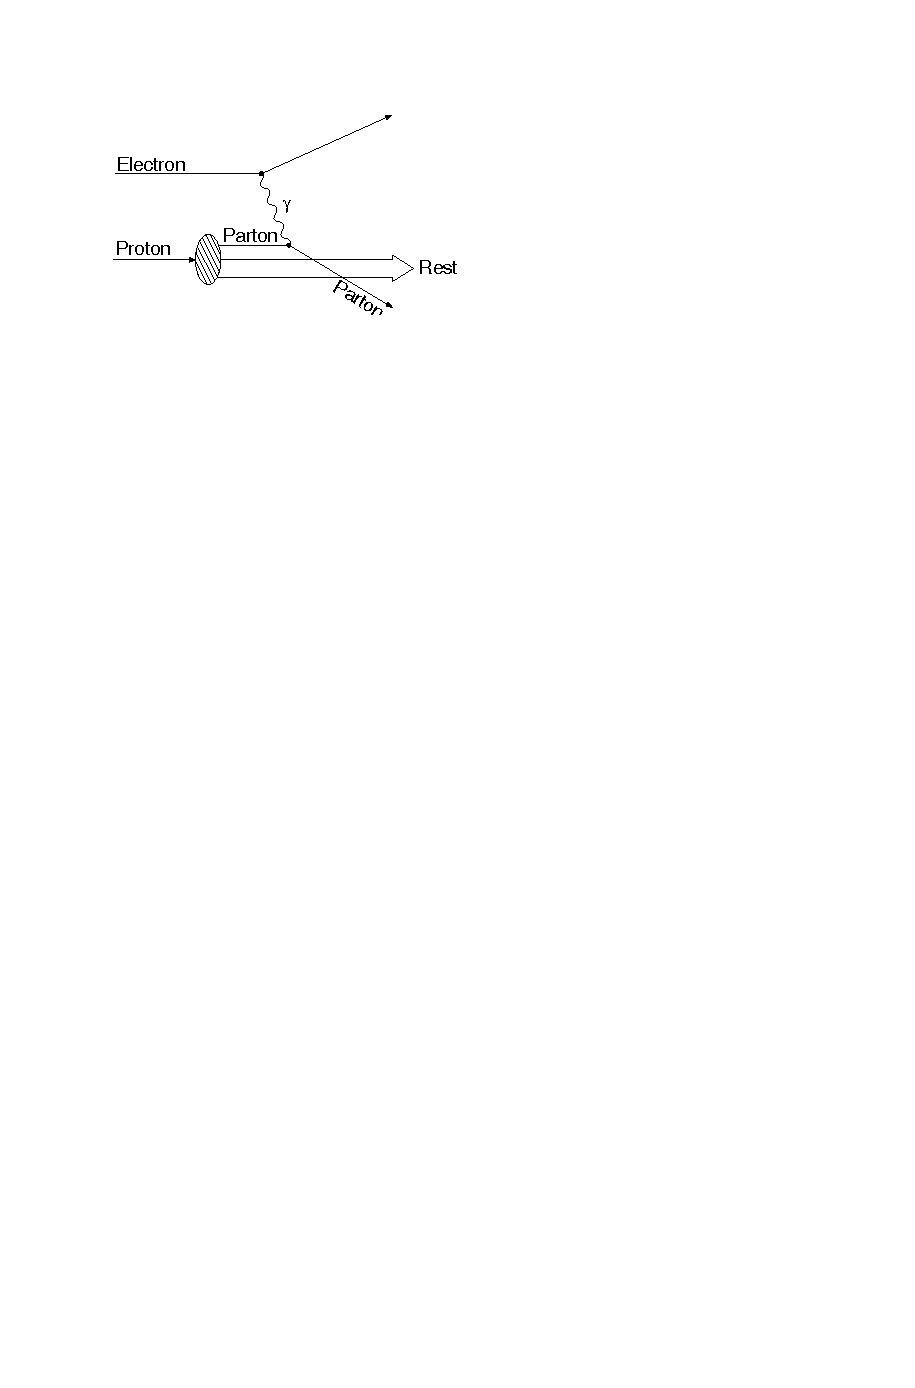
\includegraphics[width=\linewidth]{img/lab_sys.pdf}
        \caption{lab frame}
        \label{fig:eic:dis_kin::lab}
    \end{subfigure}
    \begin{subfigure}{0.48\linewidth}
        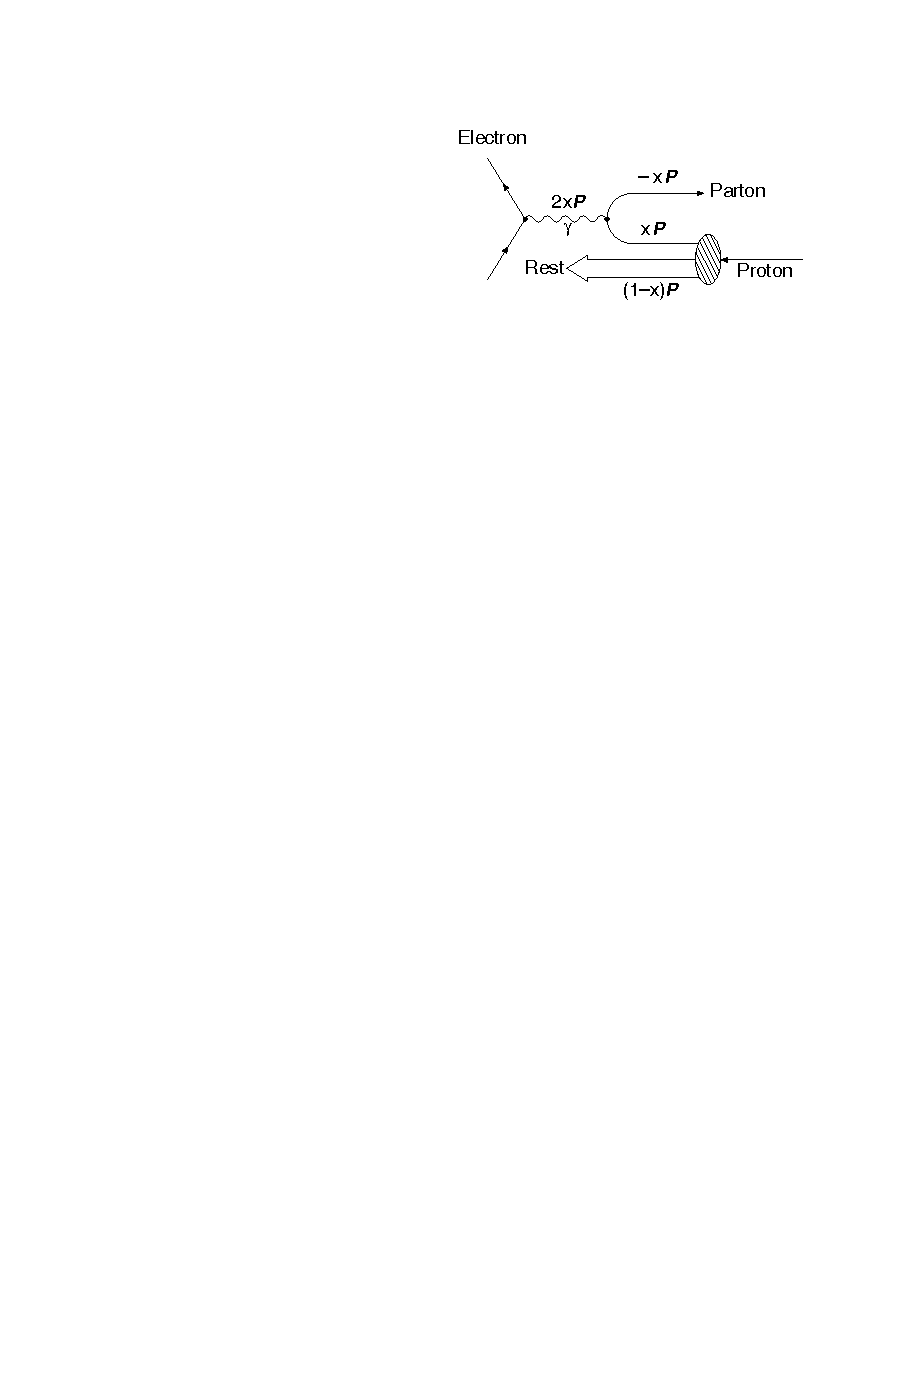
\includegraphics[width=\linewidth]{img/breit_sys.pdf}
        \caption{breit frame}
        \label{fig:eic:dis_kin::breit}
    \end{subfigure}
    \caption{[cite particles]}
    \label{fig:eic:dis_kin}
\end{figure}


Inclusive DIS

Exclusive DIS

SIDIS (previously at HERMES and COMPASS)

PDFs, GPDs

\begin{figure}[H]
    \centering
    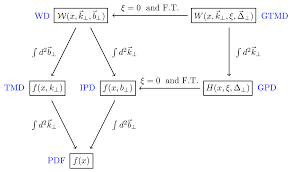
\includegraphics[width=.7\linewidth]{img/landscape.png}
    \caption{[cite landscape]}
    \label{fig:physics:landscape}
\end{figure}

scaling (pointlikeness), scaling violation

Callan-Gross (spin 1/2)

Bjorken scaling violation - dependence on Q2 at low x

\begin{figure}[H]
    \centering
    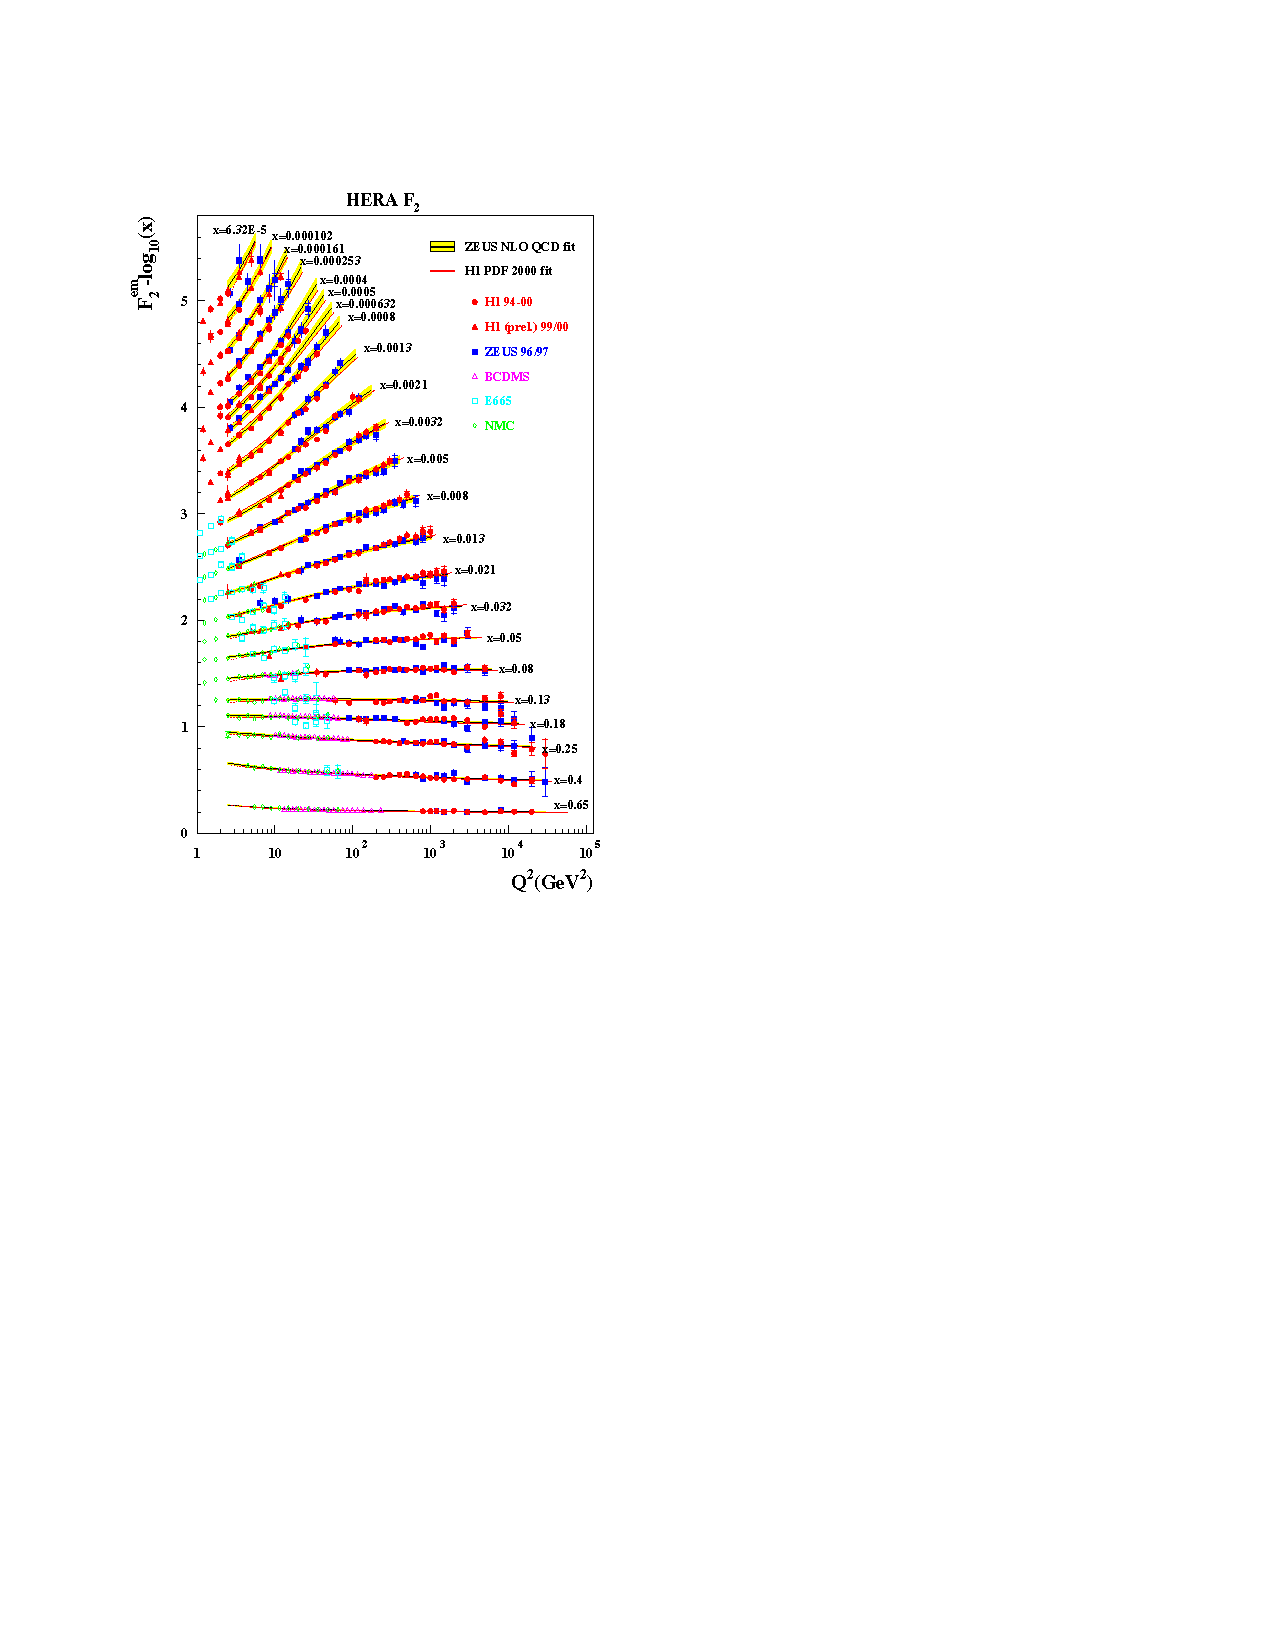
\includegraphics[width=.7\linewidth]{img/scaling_violation.pdf}
    \caption{[cite scaling violation]}
    \label{fig:physics:scaling_violation}
\end{figure}


\section{Multi-Dimensional Imaging of the Nucleon}


[YR, 29] Inclusive DIS provides a 1-dimensional picture of the nucleon as it reveals the x-distribution of (longitudinal) parton momenta in the direction of the nucleon momentum. However, due to confinement, the partons also have nonzero momenta in the (transverse) plane perpendicular to the nucleon momentum. The 3D parton structure of hadrons in momentum space is encoded in transverse momentum dependent parton distributions (TMDs). For both quarks and gluons inside a spin-1/2 hadron, a total of 8 leading-twist TMDs exist. These functions of different correlations between spins and transverse momenta reveal different insights into the dynamics of nucleons. TMDs can be measured via certain semi-inclusive processes, such as semi-inclusive DIS (SIDIS), where one detects an identified hadron in addition to the scattered lepton.

\begin{figure}[H]
    \centering
    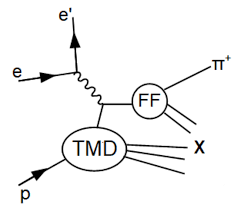
\includegraphics[width=.5\linewidth]{img/TMD_FF.png}
    \caption{placeholder [cite JLab TMD-FF]}
    \label{fig:physics:TMD_FF}
\end{figure}

\subsection{DVCS}
Deeply Virtual Compton Scattering (DVCS) is the simplest hard exclusive process related to Generalized Parton Distributions (GPDs): the scattering of an electron off a proton through the exchange of a photon of virtuality Q2, accompanied by the re-emission of a real photon

\begin{figure}[H]
    \centering
    \includegraphics[width=.5\linewidth]{img/DVCS.png}
    \caption{placeholder [cite DVCS]}
    \label{fig:physics:DVCS}
\end{figure}


Generalized Parton Distributions in ePIC, 

\section{Diffractive vector-meson production}

\begin{figure}[H]
    \centering
    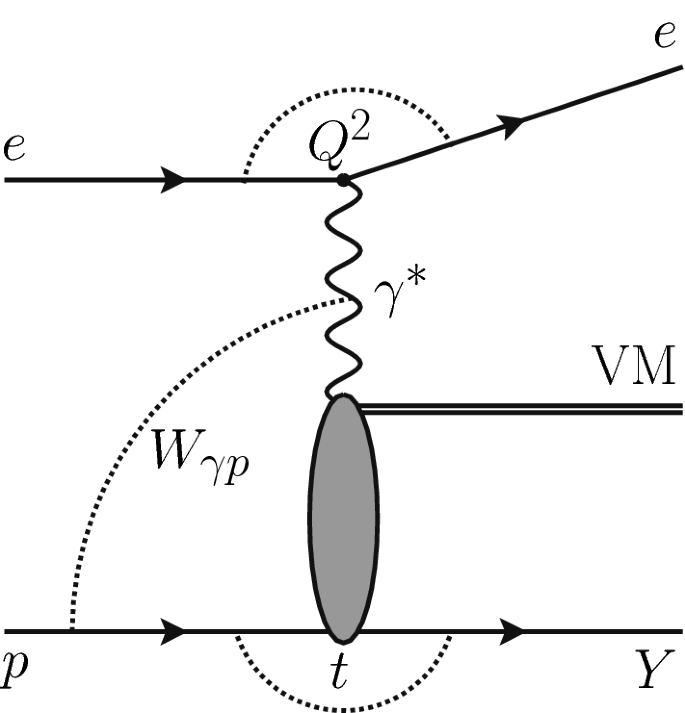
\includegraphics[width=.5\linewidth]{img/vm.png}
    \caption{placeholder [cite vm]}
    \label{fig:physics:VM}
\end{figure}

